\begin{figure}[htbp]
\centering
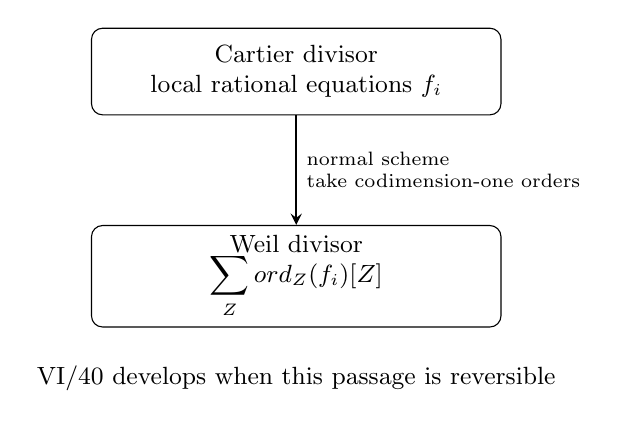
\begin{tikzpicture}[>=stealth,every node/.style={font=\small}]
\node[draw,rounded corners,minimum width=5.2cm,minimum height=1.1cm,align=center] (c) at (0,1.3) {Cartier divisor\\local rational equations $f_i$};
\node[draw,rounded corners,minimum width=5.2cm,minimum height=1.1cm,align=center] (w) at (0,-1.3) {Weil divisor\\$\displaystyle\sum_Z\operatorname{ord}_Z(f_i)[Z]$};
\draw[->,thick] (c)--node[right,align=left,font=\scriptsize]{normal scheme\\take codimension-one orders}(w);
\node at (0,-2.6) {VI/40 develops when this passage is reversible};
\end{tikzpicture}
\caption{Preview of the Cartier-to-Weil construction on a normal integral scheme.}
\label{fig:vi39-cartier-weil}
\end{figure}
